\chapter{Data retrieval and annotation}
\label{ch:retrievalannotation}


Traditionally, many corpus-linguistic studies use the (orthographic) word form as their starting point. This is at least in part due to the fact that corpora consist of text that is represented as a sequence of word forms, and that, consequently, word forms are easy to retrieve. As briefly discussed in Chapter \ref{ch:corpuslinguistics}, concordancing software allows us to query the corpus for a string of characters and displays the result as a list of hits in context.

As we saw when discussing the case of \textit{pavement} in Chapter \ref{ch:scientificmethod}, a corpus query for a string of characters like $\langle$ \texttt{pavement} $\rangle$ may give us more than we want -- it will return not only hits corresponding to the word sense ``pedestrian footpath'', which we could contrast with the synonym \textit{sidewalk}, but also those corresponding to the word sense ``hard surface'' (which we could contrast with the synonym \textit{paving}).

The query may, at the same time, give us \emph{less} than we want, because it would only return the singular form of the word and only if it is spelled entirely in lower-case. A study of the word (in either or both of its senses) would obviously require that we look at the \emph{lemma} PAVEMENT, comprising at least the word forms \textit{pavement} (singular), \textit{pavements} (plural) and, depending on how the corpus is prepared, \textit{pavement's} (possessive). It also requires that we include in our query all possible graphemic variants, comprising at least cases in lower case, with an initial capital (\textit{Pavement, Pavements, Pavement's}, e.g. at the beginning of a sentence), or in all caps (\textit{PAVEMENT, PAVEMENTS, PAVEMENT'S)}, but, depending on the corpus, also hyphenated cases occurring at a line break (e.g. \textit{pave-}$\P$\textit{ment}, with $\P$ standing for the line break).

In Chapter \ref{ch:scientificmethod}, we implicitly treated the second issue as a problem of \textit{retrieval}, noting in passing that we queried our corpus in such a way as to capture all variants of the lemma PAVEMENT. We treated the first issue as a problem of categorization -- we went through the results of our query one by one, determining from the context, which of the senses of \textit{pavement} we were likely dealing with. In the context of a research project, our decisions would be recorded together with the data in some way -- we would \emph{annotate} the data, using an agreed-upon \emph{code} for each of the categories (e.g., word senses).

Retrieval is a non-trivial issue even when dealing with individual lexical items whose orthographic representations are not ambiguous. The more complex the phenomena under investigation are, the more complex these issues become, requiring careful thought and a number of decisions concerning an almost inevitable trade-off between the quality of the results and the time needed to retrieve them. This issue will be dealt with in Section \ref{sec:retrieval}. We already saw that the issue of annotating the data is extremely complex even in the case of individual lexical items. and the preceding chapter discussed some more complicated examples. This issue will be dealt with in more detail in Section \ref{sec:annotating}.

\section{Retrieval}
\label{sec:retrieval}

Roughly speaking, there are two ways of searching a corpus for a particular linguistic phenomenon: manually (i.e., by reading the texts contained in it, noting down each instance of the phenomenon in question) or automatically (i.e., by using a computer program to run a query on a machine-readable version of the texts). As discussed in Chapter \ref{ch:corpuslinguistics}, there may be cases where there is no readily apparent alternative to a fully manual search, and we will come back to such cases below.

However, as also discussed in Chapter \ref{ch:corpuslinguistics}, software-aided queries are the default in modern corpus linguistics, and so we take these as a starting point of our discussion.

\subsection{Corpus queries}
\label{sec:corpusqueries}

There is a range of more or less specialized commercial and non-commercial concordancing programs designed specifically for corpus linguistic research, and there are many other software packages that may be repurposed to the task of searching text corpora even though they are not specifically designed for corpus-linguistic research Finally, there are scripting languages like Perl, Python and R, with a learning curve that is not forbiddingly steep, that can be used to write programs capable of searching text corpora (ranging from very simple two-liners to very complex solutions). Which of these solutions are available to you and suitable to your research project is not for me to say, so the following discussion will largely abstract away from such specifics.

The power of software-aided searches depends on two things: on the annotation contained in the corpus itself and on the pattern-matching capacities of the software used to access them. In the simplest case (which we assumed to hold in the examples discussed in the previous chapter), a corpus will contain plain text in a standard orthography and the software will be able to find passages matching a specific string of characters. Essentially, this is something every word processor is capable of. 

Most concordancing programs (and many other types of computer programs) can do more than this, however. For example, they typically allow the researcher to formulate queries that match not just one string, but a class of strings. One fairly standardized way of achieving this is by using so-called ``regular expressions'' -- strings that may contain not just simple characters, but also symbols referring to classes of characters or symbols affecting the interpretation of characters. For example, the lexeme \textit{sidewalk}, has (at least) six possible orthographic representations: \textit{sidewalk}, \textit{side-walk}, \textit{Sidewalk}, \textit{Side-walk}, \textit{sidewalks}, \textit{side-walks}, \textit{Sidewalks} and \textit{Side-walks} (in older texts, it is sometimes spelled as two separate words, which means that we have to add at least \textit{side walk}, \textit{side walks}, \textit{Side walk} and \textit{Side walks} when investigating such texts). In order to retrieve all occurrences of the lexeme, we could perform a separate query for each of these strings, but I actually queried the string in (\ref{ex:regexexample}a); a second example of regular expressions is (\ref{ex:regexexample}b), which represents one way of searching for all inflected forms and spelling variants of the verb \textit{synthesize} (as long as they are in lower case):

\begin{exe}
\ex
\begin{xlist} 
\label{ex:regexexample}
\ex \texttt{[Ss]ide[- ]?walks?}
\ex \texttt{synthesi[sz]e?[ds]?(ing)?}
\end{xlist}
\end{exe}

Any group of characters in square brackets is treated as a class, meaning that any one of them will be treated as a match, and the question mark means ``zero or one of the preceding characters''). This means, that the pattern in (5.1a) will match an upper- or lower-case \textit{S}, followed by \textit{i}, \textit{d}, and \textit{e}, followed by zero or one occurrence of a hyphen or a blank space, followed by \textit{w}, \textit{a}, \textit{l}, and \textit{k}, followed by zero or one occurrence of \textit{s}. This matches all the variants of the word. For \ref{ex:regexexample}b), the [sz] ensures that both the British spelling (with an \textit{s}) and the American spelling (with a \textit{z}) are found. The question mark after \textit{e} ensures that both the forms with an \textit{e} (\textit{synthesize, synthesizes, synthesized}) and that without one (\textit{synthesizing}) are matched. Next, the sting matches zero to one occurrence of a \textit{d} or an \textit{s} followed by zero or one occurrence of the string \textit{ing} (because it is enclosed in parentheses, it is treated as a unit for the purposes of the following question mark.

Regular expressions allow us to formulate the kind of complex and abstract  queries that we are likely to need when searching for words (rather than individual word forms) and even more so when searching for more complex expressions. But even the simple example in (\ref{ex:regexexample}) demonstrates a problem with such queries: they quickly overgeneralize. The pattern would also, for example, match some non-existing forms, like \textit{synthesizding}, and, more crucially, it will match existing forms that we may not want to include in our search results, like the noun \textit{synthesis} (see further Section \ref{sec:precisionrecall}).

The benefits of being able to define complex queries becomes even more obvious if our corpus contains annotations in addition to the original text, as discussed in Chapter \ref{ch:corpuslinguistics} in Section \ref{sec:annotations}. If the corpus contains part-of-speech tags, for example, this will allow us to search (within limits) for grammatical structures. For example, assume that there is a part-of-speech tag attached to the end of every word by an underscore (as in the BROWN corpus, see example (\ref{fig:brownstructfeatures}) in Chapter \ref{ch:corpuslinguistics}) and that the tags are as shown in (\ref{ex:browntags}) (following the sometimes rather nontransparent BROWN naming conventions). We could then search for prepositional phrases using a pattern like the one in (\ref{ex:npqueryregex}):

\begin{exe}
\ex
\begin{tabular}[t]{ll}
preposition & \texttt{\_IN}\\
articles & \texttt{\_AT}\\
adjectives & \texttt{\_JJ} (uninflected)\\
 & \texttt{\_JJR} (comparative)\\
 & \texttt{\_JJT} (superlative)\\
nouns & \texttt{\_NN} (common singular nouns)\\
 & \texttt{\_NNS} (common plural nouns)\\
 & \texttt{\_NN\$} (common nouns with possessive clitic)\\
 & \texttt{\_NP} (proper names)\\
 & \texttt{\_NP\$} (proper nouns with possessive clitic)
\end{tabular}
\label{ex:browntags}
\end{exe}

\begin{exe}
\ex
\begin{tabular}[t]{cccc}
\texttt{\textbackslash{}S+\_IN} & \texttt{(\textbackslash{}S+\_AT)?} & \texttt{(\textbackslash{}S+\_JJ[RT]?)*} & \texttt{(\textbackslash{}S+\_N[PN][S\$]?)+}\\
1 & 2 & 3 & 4
\end{tabular}
\label{ex:npqueryregex}
\end{exe}

An asterisk means ``zero or more'', a plus means ``one or more'', and \textbackslash{}S means ``any non-whitespace character'', the meaning of the other symbols is as before. The pattern in (\ref{ex:npqueryregex}) matches the following sequence:

\begin{enumerate}
\item any word (i.e., sequence of non-whitespace characters) tagged as a preposition, followed by 
\item zero or one occurrence of a word tagged as an article that is preceded by a whitespace, followed by
\item zero or more occurrences of a word tagged as an adjective (again preceded by a whitespace), including comparatives and superlatives -- note that the JJ-tag may be followed by zero or one occurrence of a \textit{T} or an \textit{R}), followed by
\item one or more words (again, preceded by a whitespace) that are tagged as a noun or proper name -- note the square bracket containing the N for common nouns and the P for proper nouns --, including plural forms and possessive forms -- note that NN or NP tags may be followed by zero or one occurrence of an S or a \$.
\end{enumerate}

The query in (\ref{ex:npqueryregex}) makes use of the annotation in the corpus (in this case, the part-of-speech tagging), but it does so in a somewhat cumbersome way by treating word forms and the tags attached to them as strings. As shown in \ref{fig:susanneannotation} in Chapter \ref{ch:corpuslinguistics}, corpora often contain multiple annotations for each word form -- part of speech, lemma, in some cases even grammatical structure. Some concordance programs, such as the widely-used open-source Corpus Workbench (including its web-based version CQPweb) \citep[cf.][]{evert_twenty-first_2011} or the Sketch Engine and its open-source variant NoSketch engine \citep[cf.][]{kilgarriff_sketch_2014} are able to ``understand'' the structure of such annotations and offer a query syntax that allows the researcher to refer to this structure directly.

The two programs just mentioned share a query syntax called \emph{CQP} (for ``Corpus Query Processor'') in the Corpus Workbench and \emph{CQL} (for ``Corpus Query Language'') in the (No)Sketch Engine. This syntax is very powerful, allowing us to query the corpus for tokens or sequences of tokens at any level of annotation. It is also very transparent: each token is represented as a value-attribute pair in square brackets, as shown in (\ref{ex:cqptoken}): 

\begin{exe}
\ex \texttt{[attribute="value"]}
\label{ex:cqptoken}
\end{exe}

The attribute refers to the level of annotation (e.g. \texttt{word}, \texttt{pos}, \texttt{lemma} or whatever else the makers of a corpus have called their annotations), the value refers to what we are looking for. For example, a query for the different forms of the word \textit{synthesize} (cf. (\ref{ex:regexexample}) above) would look as shown in (\ref{ex:cqpexample}a), or, if the corpus contains information about the lemma of each word form, as shown in \ref{ex:cqpexample}b), and the query for NPs in \ref{ex:npqueryregex} would look as shown in (\ref{ex:cqpexample}c):

\begin{exe}
\ex
\begin{xlist} 
\label{ex:cqpexample}
\ex \texttt{[word="synthesi[sz]e?[ds]?(ing)?"]}
\ex \texttt{[lemma="synthesize"]}
\ex \texttt{[pos="IN"]} \texttt{[pos="AT"]?} \texttt{[pos="JJ[RT]"]\*} \texttt{[pos="N[PN][S\$]?"]+}
\end{xlist}
\end{exe}

As you can see, we can use regular expressions inside the values for the attributes, and we can use the asterisk, question mark and plus outside the token to indicate that the query should match ``zero or more'', ``zero or one'' and ``one or more'' tokens with the specified properties. Note that CQP syntax is case sensitive, so for example (\ref{ex:cqpexample}a) would only return hits that are in lowecase. If we want the query to be case-insensitive, we have to attach \texttt{\%c} to the value.

We can also combine two or more attribute-value pairs inside a pair of square brackets to search for tokens satisfying particular conditions at different levels of annotation. For example, (\ref{ex:cqpmoreexample}a) will find all instances of the word form \textit{walk} tagged as a verb, while (\ref{ex:cqpmoreexample}b) will find all instances tagged as a noun. We can also address different levels of annotation at different positions in query. For example, (\ref{ex:cqpmoreexample}c) will find all instances of the word form \textit{walk} followed by a word tagged as a preposition, and (\ref{ex:cqpmoreexample}d) corresponds to the query $\langle$ \texttt{through the NOUN of POSS.PRON car} $\rangle$ mentioned in Section \ref{sec:statinghypotheses} in Chapter \ref{ch:scientificmethod} (note the \texttt{\%c} that makes all queries for words case insensitive):


\begin{exe}
\ex
\begin{xlist} 
\label{ex:cqpmoreexample}
\ex \texttt{[word="walk"\%c \& pos="VB"]}
\ex \texttt{[word="walk"\%c \& pos="NN"]}
\ex \texttt{[word="walk"\%c]} \texttt{[pos="IN"]}
\ex \begin{minipage}[t]{0.85\textwidth} \raggedright \texttt{[word="through"\%c]} \texttt{[word="the"\%c]} \texttt{[pos="NNS?"]} \texttt{[word="of"\%c]} \texttt{[pos="PP\$"]} \texttt{[word="car"\%c]} \end{minipage}
\end{xlist}
\end{exe}

This query syntax is so transparent and widely-used that we will treat it as a standard in the remainder of the book and use it to describe queries. This is obviously useful if you are using one of the systems mentioned above, but if not, the transparency of the syntax should allow you to translate the query into whatever possibilities your concordancer offers you. When talking about a query in a particular corpus, I will use the annotation (e.g., the part-of-speech tags) used in that corpus, when talking about queries in general, I will use generic values like \textit{noun} or \textit{prep.}, shown in lower case to indicate that they do not correspond to a particular corpus annotation.

Of course, even the most powerful query syntax can only work with what is there. If our corpus has no syntactic annotation, even a complex query like that in \ref{ex:cqpexample} (and \ref{ex:npqueryregex}) will not return all prepositional phrases. For example, these queries will not match cases where the adjective is preceded by one or more quantifiers (tagged \texttt{\_QT} in the BROWN corpus), adverbs (tagged \texttt{\_RB}), or combinations of the two. It will also not return cases with pronouns instead of nouns. These and other issues can be fixed by augmenting the query accordingly, although the increasing complexity will bring problems of its own, to which we return in the next subsection.

Other problems are impossible to fix; for example, if the noun phrase inside the PP contains another PP, the pattern will not recognize it as belonging to the NP but will treat it as a new match and there is nothing we can do about this, since there is no difference between the sequence of POS tags in a structures like (\ref{ex:ppattachment}a), where the PP \textit{off the kitchen} is a complement of the noun \textit{room} and as such is part of the NP inside the first PP, and (\ref{ex:ppattachment}b), where the PP \textit{at a party} is an adjunct of the verb \textit{standing} and as such is not part of the NP preceding it:

\begin{exe}
\ex
\begin{xlist} 
\label{ex:ppattachment}
\ex A mill stands \textit{in a room off the kitchen}. (BROWN F04)
\ex He remembered the first time he saw her, standing \textit{across the room at a party}. (BROWN P28)
\end{xlist}
\end{exe}

In order to distinguish these cases in a query, we need a corpus annotated not just for parts of speech but also for grammatical structure (sometimes referred to as a \textit{treebank}), like the SUSANNE corpus briefly discussed in Chapter \ref{ch:corpuslinguistics}, Section \ref{sec:annotations} above.


\subsection{Precision and recall}
\label{sec:precisionrecall}

In arriving at the definition of corpus linguistics adopted in this book, we stressed the need to investigate linguistic phenomena exhaustively, which we took to mean ``taking into account all examples of the phenomenon in question'' (cf. Chapter \ref{ch:corpuslinguistics}). In order to take into account all examples of a phenomenon, we have to retrieve them first. However, as we saw in the preceding section and in Chapter \ref{ch:scientificmethod}, it is not always possible to define a corpus query in a way that will retrieve all and only the occurrences of a particular phenomenon. Instead, a query can have four possible outcomes: it may

\begin{enumerate}
\item include hits that are instances of the phenomenon we are looking for (these are referred to as a \textit{true positives} or \textit{hits}, but note that we are using the word \textit{hit} in a broader sense to mean ``anything returned as a result of a query'');
\item include hits that are not instances of our phenomenon (these are referred to as a \textit{false positives});
\item fail to include instances of our phenomenon (these are referred to as a \textit{false negatives} or \textit{misses}); or
\item fail to include strings that are not instance of our phenomenon (this is referred to as a \textit{true negative}).
\end{enumerate}

Table \ref{tab:queryoutcomes} summarizes these outcomes ($\lnot$ stands for ``not'').

\begin{table}[!htbp]
\caption{Four possible outcomes of a corpus query for a phenomenon X}
\label{tab:queryoutcomes}
\begin{tabular}[t]{lrcc}
\lsptoprule
       &         & \multicolumn{2}{c}{Search result} \\
       &         & Included   & Not included       \\
\midrule
Corpus  &  X     & \makecell[t]{True positive \\ \footnotesize{(\textit{hit})}}  &  \makecell[t]{False negative \\ \footnotesize{(\textit{miss})}} \\
        &  $\lnot$ X & \makecell[t]{False positive \\ \footnotesize{(\textit{false alarm})}}         &  \makecell[t]{True negative \\ \footnotesize{(\textit{correct rejection})}} \\
\lspbottomrule
\end{tabular}
\end{table}

Obviously, the first case (true positive) and the fourth case (true negative) are desirable outcomes: we want our search results to include all instances of the phenomenon under investigation and exclude everything that is not such an instance. The second case (false negative) and the third case (false positive) are undesirable outcomes: we do not want our query to miss instances of the phenomenon in question and we do not want our search results to incorrectly include strings that are not instances of it.

We can describe the quality of a data set that we have retrieved from a corpus in terms of two measures. First, the proportion of positives (i.e., strings returned by our query) that are true positives; this is referred to as \textit{precision} (or as the \textit{positive predictive value}, cf. \ref{ex:precisionrecall}a). Second, the proportion of all instances of our phenomenon that are true positives (i.e., that were actually returned by our query; this is referred to as \textit{recall} (cf. \ref{ex:precisionrecall}b):\footnote{There are two additional measures that are important in other areas of empirical research but do not play a central role in corpus-linguistic data retrieval. First, the \emph{specificity} or true negative rate -- the proportion of negatives that are incorrectly included in our data (i.e. false negatives); second, \emph{negative predictive value} -- the proportion of negatives (i.e., cases not included in our search) that are true negatives (i.e., that are correctly rejected). These measures play a role in situations where a negative outcome of a test is relevant (for example, with medical diagnoses); in corpus linguistics, this is generally not the case. There are also various scores that combine individual measures to give us an overall idea of the accuracy of a test, for example, the \emph{F1 score}, defined as the harmonic mean of precision and recall. Such scores are useful in information retrieval or machine learning, but less so in corpus-linguistic research projects, where precision and recall must typically be assessed independently of, and weighed against, each other.}

\begin{exe}
\ex
\begin{xlist} 
\label{ex:precisionrecall}
\ex $\displaystyle{\text{Precision} = \frac{\text{True Positives}}{\text{True Positives} + \text{False Positives}}}$\\
\ex $\displaystyle{\text{Recall} = \frac{\text{True Positives}}{\text{True Positives} + \text{False Negatives}}}$
\end{xlist}
\end{exe}

Ideally, the value of both measures should be 1, i.e., our data should include all cases of the phenomenon under investigation (a recall rate of 100 percent) and it should include nothing that is not a case of this phenomenon (a precision of 100 percent). However, unless we carefully search our corpus manually (a possibility I will return to below), there is typically a trade-off between the two. Either we devise a query that matches only clear cases of the phenomenon we are interested in (high precision) but that will miss many less clear cases (low recall). Or we devise a query that matches as many potential cases as possible (high recall), but that will include many cases that are not instances of our phenomenon (low precision).

Let us look at a specific example, the English ditransitive construction, and let us assume that we have an untagged and unparsed corpus. How could we retrieve instances of the ditransitive? As the first object of a ditransitive is usually a pronoun (in the objective case) and the second a lexical NP (see, for example, \citet{thompson_iconicity_1987}), one possibility would be to search for a pronoun followed by a determiner (i.e., for any member of the set of strings in (\ref{ex:ditransitivequery}a)), followed by any member of the set of strings in (\ref{ex:ditransitivequery}b)). This gives us the query in (\ref{ex:ditransitivequery}c), which is long, but not very complex:

\begin{exe}
\ex
\begin{xlist} 
\label{ex:ditransitivequery}
\ex \textit{me}, \textit{you}, \textit{him}, \textit{her}, \textit{it}, \textit{us}, \textit{them}
\ex \textit{the}, \textit{a}, \textit{an}, \textit{this}, \textit{that}, \textit{these}, \textit{those}, \textit{some}, \textit{many}, \textit{lots}, \textit{my}, \textit{your}, \textit{his}, \textit{her}, \textit{its}, \textit{our}, \textit{their}, \textit{something}, \textit{anything}
\ex \begin{minipage}[t]{0.85\textwidth} \raggedright \texttt{[word="(me|\allowbreak you|\allowbreak him|\allowbreak her|\allowbreak it|\allowbreak us|\allowbreak them)"\%c]} \texttt{[word="(the|\allowbreak a|\allowbreak an|\allowbreak this|\allowbreak that|\allowbreak these|\allowbreak those|\allowbreak some|\allowbreak many|\allowbreak lots|\allowbreak my|\allowbreak your|\allowbreak his|\allowbreak her|\allowbreak its|\allowbreak our|\allowbreak their|\allowbreak something|\allowbreak anything)"\%c]} \end{minipage}
\end{xlist}
\end{exe}

Let us apply this query (which is actually used in \citet{colleman_constructional_2011}) to a freely available sample from the ICE-GB mentioned above. This corpus has been manually annotated, amongst other things, for argument structure, so that we can check the results of our query against this annotation.

There are 36 ditransitive clauses in the sample, thirteen of which are returned by our query. There are also 2838 clauses that are not ditransitive, 14 of which are also returned by our query. Table \ref{tab:queryoutcomesexample} shows the results of the query in terms of true and false positives and negatives:

\begin{table}[!htbp]
\caption{Comparison of the search results}
\label{tab:queryoutcomesexample}
\begin{tabular}[t]{lrccr}
\lsptoprule
       &         & \multicolumn{2}{c}{Search result} & \\
       &         & Included & Not included  & Total     \\
\midrule
Corpus  &  Ditransitive     & \makecell[t]{13 \\ \footnotesize{\textit{true positives}}}  &  \makecell[t]{23 \\ \footnotesize{\textit{false negatives}}} & 36 \\
        &  $\lnot$ Ditransitive & \makecell[t]{14 \\ \footnotesize{\textit{false positives}}}         &  \makecell[t]{2824 \\ \footnotesize{\textit{true negatives}}} & 2838 \\
\midrule
 & Total & 27 & 2847 & 2874 \\
\lspbottomrule
\end{tabular}
\end{table}

We can now calculate precision and recall rate of our query:

\begin{exe}
\ex
\begin{xlist} 
\label{ex:precisionrecallrate}
\ex $\displaystyle{Precision = \frac{13}{27} = 0.48}$\\
\ex $\displaystyle{Recall = \frac{13}{36} = 0.36}$ 
\end{xlist}
\end{exe}

Clearly, neither precision nor recall are particularly impressive. Let us look at the reasons for this, beginning with precision.

While the sequence of a pronoun and a determiner is typical for (one type of) ditransitive clause, it is not unique to the ditransitive, as the following false positives of our query show:

\begin{exe}
\ex
\begin{xlist} 
\label{ex:ditrfalsepositives}
\ex ... one of the experiences that went towards making me a Christian...
\ex I still ring her a lot.
\ex I told her that I 'd had to take these tablets
\ex It seems to me that they they tend to come from
\ex Do you need your caffeine fix before you this
\end{xlist}
\end{exe}

Two other typical structures characterized by the sequence pronoun\hyp{}determiner are object\hyp{}complement clauses (cf. \ref{ex:ditrfalsepositives}a) and clauses with quantifying noun phrases (cf. \ref{ex:ditrfalsepositives}b). In addition, some of the strings in (\ref{ex:ditransitivequery}b) above are ambiguous, i.e., they can represent parts of speech other than determiner; for example, \textit{that} can be a conjunction, as in (\ref{ex:ditransitivequery}c), which otherwise fits the description of a ditransitive, and in (\ref{ex:ditrfalsepositives}d), which does not. Finally, especially in spoken corpora, there may be fragments that match particular search criteria only accidentally (cf. \ref{ex:ditrfalsepositives}e). Obviously, a corpus tagged for parts of speech could improve the precision of our search results somewhat, by excluding cases like (\ref{ex:ditransitivequery}c-d), but others, like (\ref{ex:ditransitivequery}a), could never be excluded, since they are identical to the ditransitive as far as the sequence of parts-of-speech is concerned.

Of course, it is relatively trivial, in principle, to increase the precision of our search results: we can manually discard all false positives, which would increase precision to the maximum value of 1. Typically, our data will have to be manually annotated for various criteria anyway, allowing us to discard false positives in the process. However, the larger our data set, the more time consuming this will become, so that precision should always be a consideration even at the stage of data retrieval.

Let us now look at the reasons for the recall rate, which is even worse than the precision. There are, roughly speaking, four types of ditransitive structures that our query misses, exemplified in (\ref{ex:ditrfalsenegatives}a--e):

\begin{exe}
\ex
\begin{xlist} 
\label{ex:ditrfalsenegatives}
\ex How much money have they given you?
\ex The centre [...] has also been granted a three-year repayment freeze.
\ex He gave the young couple his blessing.
\ex They have just given me enough to last this year.
\ex He finds himself [...] offering Gradiva flowers.
\end{xlist}
\end{exe}

The first group of cases are those where the second object does not appear in its canonical position, for example in interrogatives and other cases of left-dislocation (cf. \ref{ex:ditrfalsenegatives}a), or passives (\ref{ex:ditrfalsenegatives}b). The second group of cases are those where word order is canonical, but either the first object (\ref{ex:ditrfalsenegatives}c) or the second object (\ref{ex:ditrfalsenegatives}d) or both (\ref{ex:ditrfalsenegatives}e) do not correspond to the query.

Note that, unlike precision, the recall rate of a query cannot be increased after the data have been extracted from the corpus. Thus, an important aspect in constructing a query is to annotate a random sample of our corpus manually for the phenomenon we are interested in, and then to check our query against this manual annotation. This will not only tell us how good or bad the recall of our query is, it will also provide information about the most frequent cases we are missing. Once we know this, we can try to revise our query to take these cases into account. In a POS-tagged corpus, we could, for example, search for a sequence of a pronoun and a noun in addition to the sequence pronoun-determiner that we used above, which would give us cases like (\ref{ex:ditrfalsenegatives}d), or we could search for forms of \textit{be} followed by a past participle followed by a determiner or noun, which would give us passives like those in (\ref{ex:ditrfalsenegatives}b).

In some cases, however, there may not be any additional patterns that we can reasonably search for. In the present example with an untagged corpus, for example, there is no additional pattern that seems in any way promising. In such cases, we have two options for dealing with low recall: First, we can check (in our manually annotated subcorpus) whether the data recalled differ from the data not recalled in any way significant for our research question. If this is not the case, we might decide to continue working with a low recall and hope that our results are still generalizable (\citet{colleman_constructional_2011}, for example, are mainly interested in the question which classes of verbs were used ditransitively at what time in the history of English, a question that they were able to discuss insightfully based on the subset of ditransitives matching their query).

If our data \textit{do} differ significantly along one or more of the dimensions relevant to our research project, we might have to increase the recall at the expense of precision and spend more time weeding out false positives. In the most extreme case, this might entail extracting the data manually, so let us return to this possibility in light of the current example. 

\subsection{Manual, semi-manual and automatic searches}
\label{sec:searchtypes}

In theory, the highest quality search results would always be achieved by a kind of close reading, i.e. a careful word-by-word (or phrase by phrase, clause by clause) inspection of the corpus. As already discussed in Chapter \ref{ch:corpuslinguistics}, this may sometimes be the only feasible option, either because automatic retrieval is difficult (as in the case of searching for ditransitives in an untagged corpus), or because an automatic retrieval is impossible (e.g., because the phenomenon we are interested in does not have any consistent formal properties, a point we will return to presently).

As discussed above, in the case of words and in at least some cases of grammatical structures, the quality of automatic searches may be increased by using a corpus annotated automatically with part-of-speech tags, phrase tags or even a grammatical structures.  As discussed in Section \ref{sec:partsofspeech} in Chapter \ref{ch:scientificmethod}, this brings with it its own problems, as automatic tagging and grammatical parsing are far from perfect. Still, an automatically annotated corpus will frequently allow us to define searches whose precision and recall are higher than in the example above.

In the case of many other phenomena, however, automatic annotation is simply not possible, or yields a quality so low that it simply does not make sense to base queries on it. For example, linguistic metaphors are almost impossible to identify automatically, as they have little or no properties that systematically set them apart from literal language. Consider the following examples of the metaphors \textsc{anger is heat} and \textsc{anger is a (hot) liquid} (from \citet{lakoff_cognitive_1987}):

\begin{exe}
\ex
\begin{xlist} 
\label{ex:angerheatnonpattern}
\ex Boy, am I burned up.
\ex He's just letting off steam.
\ex I had reached the boiling point.
\end{xlist}
\end{exe}

The first problem is that while the expressions in (\ref{ex:angerheatnonpattern}a-c) may refer to feelings of anger or rage, they can also occur in their literal meaning, as the corresponding authentic examples in (\ref{ex:literalheatnopattern}a--c) show:

\begin{exe}
\ex
\begin{xlist} 
\label{ex:literalheatnopattern}
\ex ``Now, after I am burned up,'' he said, snatching my wrist, ``and the fire is out, you \textit{must} scatter the ashes. ..." (Anne Rice, \textit{The Vampire Lestat})
\ex As soon as the driver saw the train which had been hidden by the curve, he let off steam and checked the engine... (Galignani, \textit{Accident on the Paris and Orleans Railway})
\ex Heat water in saucepan on highest setting until you reach the boiling point and it starts to boil gently. (www.sugarfreestevia.net)
\end{xlist}
\end{exe}

Obviously, there is no query that would find the examples in (\ref{ex:angerheatnonpattern}) but not those in (\ref{ex:literalheatnopattern}). In contrast, it is very easy for a human to recognize the examples in (\ref{ex:literalheatnopattern}) as literal. If we are explicitly interested in metaphors involving liquids and/or heat, we could choose a semi-manual approach, first extracting all instances of words from the field of liquids and/or heat and then discarding all cases that are not metaphorical. This type of approach is used quite fruitfully, for example, by \citet{deignan_metaphor_2005}, amongst others.

If we are interested in metaphors of anger in general, however, this approach will not work, since we have no way of knowing beforehand which semantic fields to include in our query. This is precisely the situation where exhaustive retrieval can only be achieved by a manual corpus search, i.e., by reading the entire corpus and deciding for each word, phrase or clause, whether it constitutes an example of the phenomenon we are looking for. Thus, it is not surprising that many corpus-linguistic studies on metaphor are based on manual searches (see, for example, \citet{semino_politics_1996} or \citet{jakel_metaphern_1997} for very thorough early studies of this type).

However, as mentioned in Chapter \ref{ch:corpuslinguistics}, manual searches are very time\hyp{}consuming and this limits their practical applicability: either we search large corpora, in which case manual searching is going to take more time and human resources than are realistically available, or we perform the search in a realistic time-frame and with the human resources realistically available, in which case we have to limit the size of our corpus so severely that the search results can no longer be considered representative of the language as a whole. Thus, manual searches are useful mainly in the context of research projects looking at a linguistic phenomenon in some clearly defined subtype of language (for example, metaphor in political speeches, see \citet{charteris-black_politicians_2005}).

When searching corpora for such hard-to-retrieve phenomena, it may sometimes be possible to limit the analysis usefully to a subset of the available data, as shown in the previous subsection, where limiting the query for the ditransitive to active declarative clauses with canonical word order still yielded potentially useful results. It depends on the phenomenon and the imagination of the researcher to find such easier-to-retrieve subsets.

To take up the example of metaphors introduced above, consider the examples in (\ref{ex:angerheatpattern}), which are quite close in meaning to the corresponding examples in (\ref{ex:angerheatnonpattern}a--c) above (also from \citet{lakoff_cognitive_1987}):

\begin{exe}
\ex
\begin{xlist} 
\label{ex:angerheatpattern}
\ex He was consumed by his anger.
\ex He was filled with anger.
\ex She was brimming with rage.
\end{xlist}
\end{exe}

In these cases, the PPs \textit{by/with anger/rage} make it clear that \textit{consume}, \textit{(be) filled} and \textit{brimming} are not used literally. If we limit ourselves just to metaphorical expressions of this type, i.e. expressions that explicitly mention both semantic fields involved in the metaphorical expression, it becomes possible to retrieve metaphors of anger semi-automatically. We could construct a query that would retrieve all instances of the lemmas ANGER, RAGE, FURY, and other synonyms of \textit{anger}, and then select those results that also contain (within the same clause or within a window of a given number of words) vocabulary from domains like ``liquids'', ``heat'', ``containers'' etc. This can be done manually by going through the concordance line by line (see, e.g., \citet{tissari_lovescapes:_2003} and \citet{stefanowitsch_happiness_2004, stefanowitsch_words_2006}, cf also Chapter \ref{ch:metaphorandmetonymy}, Section \ref{sec:targetdomains}), or automatically by running a second query on the results of the first (or by running a complex query for words from both semantic fields at the same time, see \citet{martin_corpus-based_2006}). The first approach is more useful if we are interested in metaphors involving any semantic domain in addition to ``anger'', the second approach is more useful (because more economical) in cases where we are interested in metaphors involving specific semantic domains.

Limiting the focus to a subset of cases sharing a particular formal feature is a feasible strategy in other areas of linguistics, too. For example, \citet{heyd_narratives_2016} wants to investigate ``narratives of belonging'' -- roughly, stretches of discourse in which members of a diaspora community talk about shared life experiences for the purpose of affirming their community membership. At first glance, this is the type of potentially fuzzy concept that should give corpus linguists nightmares, even after \citet[292]{heyd_narratives_2016} operationalizes it in terms of four relatively narrow criteria that the content of a stretch of discourse must fulfill in order to count as an example. Briefly, it must refer to experiences of the speaker themselves, it must mention actual specific events, it must contain language referring to some aspect of migration, and it must contain an evaluation of the events narrated). Obviously it is impossible to search a corpus based on these criteria. Therefore, Heyd chooses a two-step strategy \citep[294]{heyd_narratives_2016}: first, she queries her corpus for the strings \emph{born in}, \emph{moved to} and \emph{grew up in}, which are very basic, presumably wide-spread ways of mentioning central aspects of one's personal migration biography, and second, she assesses the stretches of discourse within which these strings occur on the basis of her criteria, discarding those that do not fulfill all four of them (this step is somewhere between retrieval and annotation).

As in the example of the ditransitive construction discussed above, retrieval strategies like those used by \citet{stefanowitsch_words_2006} and \citet{heyd_narratives_2016} are useful where we can plausibly argue -- or better yet, show -- that the results are comparable to the results we would get if we extracted the phenomenon completely.

In cases, where the phenomenon in question does not have any consistent formal features that would allow us to construct a query, and cannot plausibly be restricted to a subset that does have such features, a mixed strategy of elicitation and corpus query may be possible. For example, \citet{levin_bathroom_2014} is interested in what they call the ``Bathroom Formula'', which he defines as ``clauses and phrases expressing speakers' need to leave any ongoing activity in order to go to the bathroom'' \citet[2]{levin_bathroom_2014}, i.e. to the toilet (sorry to offend American sensitivities\footnote{See \citet{manning_words_1974}, who shows that the word \textit{toilet} is very upsetting even to American college students.}). This speech act is realized by phrases as diverse as (\ref{ex:bathroomformula}a--c):

\begin{exe}
\ex
\begin{xlist} 
\label{ex:bathroomformula}
\ex I need a pee. (BNC A74)
\ex I have to go to the bathroom. (BNC CEX)
\ex I'm off to powder my nose. (BNC FP6)
\end{xlist}
\end{exe}

There is no way to search for these expressions (and others with the same function) unless you are willing to read through the entire BNC -- or unless you already know what to look for. \citet{levin_bathroom_2014} chooses a strategy based on the latter: he first assembles a list of expressions from the research literature on euphemisms and complement this by asking five native speakers for additional examples. He then searches for these phrases and analyzes their distribution across varieties and demographic variables like gender and class/social stratum.

Of course, this query will miss any expressions that were not part of their initial list, but the \emph{distribution} of those expressions that are included may still yield interesting results -- we can still learn something about which of these expressions are preferred in a particular variety, by a particular group of speakers, in a particular situation, etc.

If we assemble our initial list of expressions systematically, perhaps from a larger number of native speakers that are representative of the speech community in question in terms of regional origin, sex, age group, educational background, etc., we should end up with a representative sample of expressions to base our query on. If we make our query flexible enough, we will likely even capture additional variants of these expressions. If other strategies are not available, this is certainly a feasible approach. Of course, this approach only works with relatively routinized types of speech events like the ``bathroom'' formula -- greetings and farewells, asking for the time, proposing marriage, etc. -- which, while they do not have any invariable formal features, do not vary infinitely either.

To sum up, it depends on the phenomenon under investigation and on the research question whether we can take an automatic or at least a semi-automatic approach or whether we have to resort to manual data extraction. Obviously, the more completely we can extract our object of research from the corpus, the better.

\section{Annotating}
\label{sec:annotating}

Once the data have been extracted from the corpus (and, if necessary, false positives have been removed), they typically have to be annotated in terms of the variables relevant for the research question. In some cases, the variables and their values will be provided externally; they may, for example, follow from the structure of the corpus itself (as in the case of \textvv{british english} vs. \textvv{american english} defined as ``occurring in the LOB corpus'' and ``occurring in the BROWN corpus'' respectively. In other cases, the variables and their values may have been operationalized in terms of criteria that can be applied objectively (as in the case of \textvv{Length} defined as ``number of letters''). In most cases, however, some degree of interpretation will be involved (as in the case of \textvv{Animacy} or the metaphors discussed above). Whatever the case, we need a annotation scheme -- an explicit statement of the operational definitions applied. Of course, such a annotation scheme is especially important in cases where interpretative judgments are involved in categorizing the data. In this case, the annotation scheme should contain not just operational definitions, but also explicit guidelines as to how these definitions should be applied to the corpus data. These guidelines must be explicit enough to ensure a high degree of agreement if different annotators (sometimes also referred to as \emph{coders} or \emph{raters} apply it to the same data. Let us look at each of these aspects in some detail.

\subsection{Annotating as interpretation}
\label{sec:annotatingasinterpretation}

First of all, it is necessary to understand that the categorization of corpus data is an interpretative process in the first place. This is true regardless of the type of category.

Even externally given categories are typically given an interpretation in the context of a specific research project. In the simplest case, this consists in accepting the operational definitions used by the makers of a particular corpus (as well as the interpretative judgments made in applying them). Take the example of \textvv{british english} and \textvv{american english} used in Chapters 3 and 4: If we accept the idea that the LOB corpus contains ``British English'' we are accepting an interpretation of language varieties that is based on geographical criteria: British English means ``the English spoken by people who live (perhaps also: who were born and grew up) in the British Isles''.

Or take the example of \textvv{Sex}, one of the demographic speaker variables included in many modern corpora: By accepting the values of this variable, that the corpus provides (typically \textvv{male} and \textvv{female}), we are accepting a specific interpretation of what it means to be ``male'' or ``female''. In some corpora, this may be the interpretation of the speakers themselves (i.e., the corpus creators may have asked the speakers to specify their sex), in other cases this may be the interpretation of the corpus creators (based, for example, on the first names of the speakers or on the assessment of whoever collected the data). For many speakers in a corpus, these different interpretations will presumably match, so that we can accept whatever interpretation was used as an approximation of our own operation definition of \textvv{Sex}. But in research projects that are based on a specific understanding of \textvv{Sex} (for example, as a purely biological, a purely social or a purely psychological category), simply accepting the (often unstated) operational definition used by the corpus creators may distort our results substantially. The same is true of other demographic variables, like education, income, social class etc., which are often defined on a ``common sense'' basis that does not hold up to the current state of sociological research.

Interpretation also plays a role in the case of seemingly objective criteria. Even though a criterion such as ``number of letters'' is largely self\hyp{}explanatory, there are cases requiring interpretative judgments that may vary across researchers. In the absence of clear instructions they may not know, among other things, whether to treat ligatures as one or two letters, whether apostrophes or word-internal hyphens are supposed to count as letters, or how to deal with spelling variants (for example, in the BNC the noun \textit{programme} also occurs in the variant \textit{program} that is shorter by two letters). This type of orthographic variation is very typical of older stages of English (before there was a somewhat standardized orthography), which causes problems not only for retrieval (cf. the discussion in Section \ref{sec:corpusqueries} above, cf. also \citet{barnbrook_language_1996}, Ch. 8.2 for more detailed discussion), but also for a reasonable application of the criterion ``number of letters''.

In such cases, the role of interpretation can be reduced by including explicit instructions for dealing with potentially unclear cases. However, we may not have thought of all potentially unclear cases before we start annotating our data, which means that we may have to amend our annotation scheme as we go along. In this case, it is important to check whether our amendments have an effect on the data we have already annotated, and to re-annotate them if necessary.

In cases of less objective criteria (such as \textvv{Animacy} discussed in Chapter \ref{ch:retrievalannotation} above), the role of interpretation is obvious. No matter how explicit our annotation scheme, we will come across cases that are not covered and will require individual decisions; and even the clear cases are always based on an interpretative judgment. As mentioned in Chapter \ref{ch:needforcorpus}, this is not necessarily undesirable in the same way that intuitive judgements about acceptability are undesirable; interpreting linguistic utterances is a natural activity in the context of using language. Thus, if our operational definitions of the relevant variables and values are close to the definitions speakers implicitly apply in everyday linguistic interactions, we may get a high degree of agreement even in the absence of an explicit annotation scheme,\footnote{In fact, it may be worth exploring, within a corpus-linguistic framework, ways of annotating data that are based entirely on implicit decisions by untrained speakers; specifically, I am thinking here of the kinds of association tasks and sorting tasks often used in psycholinguistic studies of word meaning.} and certainly, operational definitions should strive to retain some degree of linguistic naturalness in the sense of being anchored in interpretation processes that plausibly occur in language processing. 

\subsection{Annotation schemes}
\label{sec:annotationschemes}

We can think of a linguistic annotation scheme as a comprehensive operational definition for a particular variable, with detailed instructions as to how the values of this variable should be assigned to linguistic data (in our case, corpus data, but of course annotation schemes are also needed to categorize experimentally elicited linguistic data). The annotation scheme would typically also include a \emph{coding scheme}, specifying the labels by which these categories are to be represented. For example, the distinctions between different degrees of ``Animacy'' need to be defined in a way that allows us to identify them in corpus data (this is the annotation scheme, cf. below), and the scheme needs to specify names for these categories (for example, the category containing animate entities could be labelled by the codes \textvv{animate}, \textvv{anim}, \textvv{\#01}, \textvv{cat:7345}, etc. -- as long as we know what the label stands for, we can choose it randomly).

In order to keep different research projects in a particular area comparable, it is of course desirable to create annotation and coding schemes independently of a particular research project. However, the field of corpus-linguistics is not well-established and methodologically mature enough yet to have yielded uncontroversial and widely applicable annotation schemes for most linguistic phenomena. There are some exceptions, such as the part-of-speech tag sets and the parsing schemes used by various wide-spread automatic taggers and parsers, which have become de facto standards by virtue of being easily applied to new data; there are also some substantial attempts to create annotation schemes for the manual annotation of phenomena like topicality \citep[cf.][]{givon_topic_1983}, animacy \citep[cf.][]{zaenen_animacy_2004}, and the grammatical description of English sentences \citep[e.g.][]{sampson_english_1995}.

Whenever it is feasible, we should use existing annotation schemes instead of creating our own -- searching the literature for such schemes should be a routine step in the planning of a research project. Often, however, such a search will come up empty, or existing annotation schemes will not be suitable for the specific data we plan to use or they may be incompatible with our theoretical assumptions. In these cases, we have to create our own annotation schemes.

The first step in creating a annotation scheme for a particular variable consists in deciding on a set of values that this variable may take. As the example of \textvv{Animacy} in Chapter \ref{ch:retrievalannotation} shows, this decision is loosely constrained by our general operational definition, but the ultimate decision is up to us and must be justified within the context of our theoretical assumptions and our specific research question.

There are, in addition, several general criteria that the set of values for any variable must meet. First, they must be non-overlapping. This may seem obvious, but it is not at all unusual, for example, to find continuous dimensions split up into overlapping categories, as in the following quotation:

\begin{quote}
Hunters aged 15--25 years old participated more in non-consumptive activities than those aged 25--35 and 45--65 (P<0.05), as were those aged 35--45 compared to those 55--65 years old (P<0.05). \citep[304]{ericsson_jagare_2002}.
\end{quote}

Here, the authors obviously summarized the ages of their subjects into the following four classes: (I) 25--35, (II) 35--45, (III) 45--55 and (IV) 55--65: thus, subjects aged 35 could be assigned to class I or class II, subjects aged 45 to class II or class III, and subjects aged 55 to class III or class IV. This must be avoided, as different annotators might make different decisions, and as other researchers attempting to replicate the research will not know how we categorized such cases.

Second, the variable should be defined such that it does not conflate properties that are potentially independent of each other, as this will lead to a set of values that do not fall along a single dimension. As an example, consider the so-called \textit{Silverstein Hierarchy} used to categorize nouns for (inherent) Topicality (after \citealt[67]{deane_english_1987}): 

\begin{exe}
\ex 1\textsuperscript{st} person pronoun\\
2\textsuperscript{nd} person pronoun\\
3\textsuperscript{rd} person pronoun\\
3\textsuperscript{rd} person demonstrative\\
Proper name\\
Kin-Term\\
Human and animate NP\\
Concrete object\\
Container\\
Location\\
Perceivable\\
Abstract
\label{ex:silverstein}
\end{exe}

Note, first, that there is a lot of overlap in this annotation scheme. For example, a first or second person pronoun will always refer to a human or animate NP and a third person pronoun will frequently do so, as will a proper name or a kin term. Similarly, a container is a concrete object and can also be a location, and everything above the category Perceivable is also perceivable. This overlap can only be dealt with by an instruction of the kind that every nominal expression should be put into the topmost applicable category; in other words, we need to add an ``except for expressions that also fit into one of the categories above'' to every category label.

Secondly, although the Silverstein Hierarchy may superficially give the impression of providing values of a single variable that could be called \textvv{Topicality}, it is actually a mixture of several quite different variables and their possible values. One attempt of disentangling these variables and giving them each a set of plausible values is the following:

\begin{exe}
\ex
\begin{xlist} 
\label{ex:silversteinuntangled}
\ex \textvv{Type of Nominal Expression}:\\
\textvv{pronoun > proper name > kinship terms > lexical np}
\ex \textvv{Discourse Role}:\\
\textvv{speaker > hearer > other (near > far)}
\ex \textvv{Animacy/Agency}:\\
\textvv{human > animate > inanimate}
\ex \textvv{Concreteness}:\\
\textvv{touchable > non-touchable concrete > abstract}
\ex \textvv{Gestalt Status}:\\
\textvv{object > container > location}
\end{xlist}
\end{exe}

Given this set of variables, it is possible to describe all categories of the Silverstein Hierarchy as a combination of values of these variables, for example:

\begin{exe}
\ex
\begin{xlist} 
\label{ex:silversteincomb}
\ex 1\textsuperscript{st} Person Pronoun:\\
\textvv{pronoun} + \textvv{speaker} + \textvv{human} + \textvv{touchable} + \textvv{object}
\ex Concrete Object:\\
\textvv{lexical np} + \textvv{other} + \textvv{inanimate} + \textvv{touchable} + \textvv{object}
\end{xlist}
\end{exe}

The set of variables in (\ref{ex:silversteinuntangled}) also allows us to differentiate between expressions that the Silverstein Hierarchy lumps together, for example, a 3\textsuperscript{rd} person pronoun could be categorized as (\ref{ex:beyondsilverstein}a), (\ref{ex:beyondsilverstein}b), (\ref{ex:beyondsilverstein}c) or (\ref{ex:beyondsilverstein}d), depending on whether it referred to a \textit{mouse}, a \textit{rock, air} or \textit{democracy}:

\begin{exe}
\ex
\begin{xlist} 
\label{ex:beyondsilverstein}
\ex \textvv{pronoun} + \textvv{other} + \textvv{animate} + \textvv{touchable} + \textvv{object}
\ex \textvv{pronoun} + \textvv{other} + \textvv{inanimate} + \textvv{touchable} + \textvv{object}
\ex \textvv{pronoun} + \textvv{other} + \textvv{inanimate} + \textvv{non-touchable} + \textvv{object} (or perhaps \textvv{location}, cf. \textit{in the air})
\ex \textvv{pronoun} + \textvv{other} + \textvv{inanimate} + \textvv{abstract} + \textvv{object} (or perhaps \textvv{location}, cf. in \textit{a democracy})
\end{xlist}
\end{exe}

There are two advantages of this more complex annotation scheme. First, it allows a more principled categorization of individual expressions: the variables and their values are easier to define and there are fewer unclear cases. Second, it would allow us to determine empirically which of the variables are actually relevant in the context of a given research question, as irrelevant variables will not show a significant distribution across different conditions. Originally, the Silverstein Hierarchy was meant to allow for a principled description of split ergative systems; it is possible, that the specific conflation of variables is suitable to this task. However, it is an open question whether the same conflation of variables is also suitable to the analysis of other phenomena. If we were to apply it as is, we would not be able to tell whether this is the case. Thus, we should always define our variables in terms of a single dimension and deal with complex concepts (like \textvv{Topicality}) by analyzing the data in terms of a set of such variables.

After defining a variable (or set of variables) and deciding on the type and number of values, the second step in creating a annotation scheme consists in defining what belongs into each category. Where necessary, this should be done in the form of a decision procedure.

For example, the annotation scheme for \textvv{Animacy} mentioned in the preceding chapter (\citealt{garretson_coding_2004}, \citealt{zaenen_animacy_2004}) has the categories \textvv{human} and \textvv{organization} (among others). The category \textvv{human} is relatively self-explanatory, as we tend to have a good intuition about what constitutes a human. Nevertheless, the annotation scheme spells out that it does not matter by what linguistic means humans are referred to (e.g., proper names, common nouns including kinship terms, and pronouns) and that dead, fictional or potential future humans are included as well as ``humanoid entities like gods, elves, ghosts, and androids''.

The category \textvv{organization} is much more complex to apply consistently, since there is no intuitively accessible and generally accepted understanding of what constitutes an organization. In particular, it needs to be specified what distinguishes an \textvv{organization} from other groups of human beings (that are to be categorized as \textvv{human} according to the annotation scheme). The annotation scheme defines an \textvv{organization} as a referent involving ``more than one human'' with ``some degree of group identity''. It then provides the following hierarchy of properties that a group of humans may have (where each property implies the presence of all properties below its position in the hierarchy):

\begin{exe}
\ex +/- chartered/official\\
+/- temporally stable\\
+/- collective voice/purpose\\
+/- collective action\\
+/- collective
\label{ex:animacyorg}
\end{exe}

It then states that ``any group of humans at + collective voice or higher'' should be categorized as \textvv{organization}, while those below should simply be annotated as \textvv{human}. By listing properties that a group must have to count as an organization in the sense of the annotation scheme, the decision is simplified considerably, and by providing a decisio6.3n procedure, the number of unclear cases is reduced. The annotation scheme also illustrates the use of the hierarchy:

\begin{quote}
Thus, while `the posse' would be an \textvv{org}, `the mob' might not be, depending on whether we see the mob as having a collective purpose. `The crowd' would not be considered \textvv{org}, but rather simply \textvv{human}.
\end{quote}

Whether or not to include such specific examples is a question that must be answered in the context of particular research projects. One advantage is that examples may help the annotators understand the annotation scheme. A disadvantage is that examples may be understood as prototypical cases against which the referents in the data are to be matched, which may lead annotators to ignore the definitions and decision procedures.

The third step, discussed in detail in the next section, consists in testing the reliability of our annotation scheme. When we are satisfied that the scheme can be reliably applied to the data, the final step is the annotation itself.

\subsection{The reliability of annotation schemes}
\label{sec:reliabilityannotationschemes}

In some cases, we may be able to define our variables in such a way that they can be annotated automatically. For example, if we define \textvv{Word Length} in terms of ``number of letters'', we could write a simple computer program to go through our corpus, count the letters in each word and attach the value as a tag. Since computers are good at counting, it would be easy to ensure that such a program is completely reliable. We could also, for example, create a list of the 2500 most frequent nouns in English and their \textvv{Animacy} values, and write a program that goes through a tagged corpus and, whenever it encounters a word tagged as a noun, looks up this value and attaches it to the word as a tag. In this case, the reliability would be much lower, as the program would not be able to distinguish between different word senses, for example assigning the label \textvv{animate} to the word \textit{horse} regardless of whether it refers to an actual horse, a hobby horse (which should be annotated as \textvv{inanimate}) or whether it occurs in the idiom \textvv{straight from the horse's mouth} (where it would presumably have to be annotated as \textvv{human}, if at all).

In these more complex cases, we can, and should, assess the quality of the automatic annotation in the same way in which we would assess the quality of the results returned by a particular query, in terms of precision and recall (cf. Section \ref{sec:precisionrecall}, Table \ref{tab:queryoutcomes}). In the context of annotating data, a true positive result for a particular value would be a case where that value has been assigned to a corpus example correctly, a false positive would be a case where that value has been assigned incorrectly, a false negative would be a case where the value has not been assigned although it should have been, and a true negative would be a case where the value has not been assigned and should not have been assigned.

This assumes, however, that we can determine with a high degree of certainty what the correct value would be in each case. The examples discussed in this chapter show, however, that this decision itself often involves a certain degree of interpretation -- even an explicit and detailed annotation scheme has to be applied by individuals based on their understanding of the instructions contained in it and the data to which they are to be applied. Thus, a certain degree of subjectivity cannot be avoided, but we need minimize the subjective aspect of interpretation as much as possible.

The most obvious way of doing this is to have (at least) two different annotators apply the annotation scheme to the data -- if our measurements cannot be made objective (and, as should be clear by now, they rarely can in linguistics), this will at least allow us to ensure that they are intersubjectively reliable.

One approach would be to have the entire data set annotated by two annotators independently on the basis of the same annotation scheme. We could then identify all cases in which the two annotators did not assign a the same value and determine, where the disagreement came from. Obvious possibilities include cases that are not covered by the annotation scheme at all, cases where the definitions in the annotation scheme are too vague to apply or too ambiguous to make a principled decision, and cases where one of the annotators has misunderstood the corpus example or made a mistake due to inattention. Where the annotation scheme is to blame, it could be revised accordingly and re-applied to all unclear cases. Where an annotator is at fault, they could correct their annotation decision. At the end of this process we would have a carefully annotated data set with no (or very few) unclear cases left.

However, in practice there are two problems with this procedure. First, it is extremely time-consuming, which will often make it difficult to impossible to find a second annotator. Second, discussing all unclear cases but not the apparently clear cases holds the danger that the former will be annotated according to different criteria than the latter.

Both problems can be solved (or at least alleviated) by testing the annotation scheme on a smaller dataset using two annotators and calculating its reliability across annotators. If this so-called interrater reliability is sufficiently high, the annotation scheme can safely be applied to the actual data set by a single annotator. If not, it needs to be made more explicit and applied to a new set of test data by two annotators; this process must be repeated until the interrater reliability is satisfactory.

A frequently used measure of interrater reliability in designs with two annotators is Cohen's $\kappa$ \citet{cohen_coefficient_1960}, which can range from 0 (``no agreement'') to 1 (``complete agreement''). It is calculated as shown in \ref{ex:cohenskappa}:\footnote{For more than two raters, there is a more general version of this metric, referred to as Fleiss' $\kappa$ \citet{fleiss_measuring_1971}, but as it is typically difficult even to find a second annotator, we will stick with the simpler measure here.}

\begin{exe}
\ex $\displaystyle{\kappa = \frac{p_o - p_e}{1 - p_e}}$
\label{ex:cohenskappa}
\end{exe}

In this formula, $p_o$ is the relative observed agreement between the raters (i.e. the percentage of cases where both raters have assigned the same category) and $p_e$ is the relative expected agreement (i.e. the percentage of cases where they should have agreed by chance).

Table \ref{tab:intterraterschematic} shows a situation where the two raters assign one of the two categories \textvv{x} or \textvv{y}. Here, $p_o$ would be the sum of \textit{n}(\textvv{x}, \textvv{x}) and \textit{n}(\textvv{y}, \textvv{y}), divided by the sum of all annotation; $p_e$ can be calculated in various ways, a straightforward one will be introduced below.

\begin{table}[!htbp]
\caption{A contingency table for two raters and two categories}
\label{tab:intterraterschematic}
\begin{tabular}[t]{llccr}
\lsptoprule
                    &                       & \multicolumn{2}{c}{\textvv{Rater 2}}                                                      \\
                    &                       & \textvv{category x}                                 & \textvv{Category x}                              \\
\midrule
\textvv{Rater 1}  & \textvv{category x} & \textit{n}(\textvv{x}, \textvv{x}) & \textit{n}(\textvv{x}, \textvv{y})\\
                  & \textvv{category y} & \textit{n}(\textvv{y}, \textvv{x}) & \textit{n}(\textvv{y}, \textvv{y})\\
\lspbottomrule
\end{tabular}
\end{table}

Let us look at a concrete example. In English, certain types of semantic relations, ``possession'' being very prominent among them, can be expressed in two alternative ways; either by the \textit{s}-possessive (traditionally referred to as ``genitive'') with the modifier marked by the clitic \textit{'s} (cf. (\ref{ex:genitivevsof}a)), or by the \textit{of}-construction, with the modifier as a prepositional object of the preposition \textit{of} (cf. (\ref{ex:genitivevsof}b):

\begin{exe}
\ex
\begin{xlist}
\label{ex:genitivevsof}
\ex a tired horse's plodding step (BROWN K13)
\ex every leaping stride of the horse (BROWN N02)
\end{xlist}
\end{exe}

Let us assume that we want to investigate the factors determining the choice between these two constructions (as we will do in Chapters \ref{ch:quantifyingresearch} and \ref{ch:significancetesting}). In order to do so, we need to identify the subset of constructions with \textit{of} that actually correspond to the \textit{s}-possessive semantically -- note that the \textit{of}-construction encodes a wide range of relations, including many -- for example quantification or partition -- that are never expressed by an \textit{s}-possessive. This means that we must manually go through the hits for the \textit{of}-construction in our data and decide whether the relation encoded could also be encoded by an \textit{s}-posessive. Let us use the term ``\textit{of}-possessive'' for these cases. Ideally, we would do this by searching a large corpus for actual examples of paraphrases with the \textit{s}-possessive, but let us assume that this is too time consuming (a fair assumption in many research contexts) and that we want to rely on introspective judgments instead.

We might formulate a simple annotation scheme like the following:

\begin{quote}
For each case of the structure [(DET\textsubscript{i}) (AP\textsubscript{i}) N\textsubscript{i} \textit{of} NP\textsubscript{j}], paraphrase it as an \textit{s}-possessove of the form [NP\textsubscript{j} \textit{'s} (APi) N\textsubscript{i}] (for example, \textit{the leaping stride of the horse} becomes \textit{the horse's leaping stride}). If the result sounds like something a speaker of English would use, assign the label \textvv{poss}, if not, assign the label \textit{other}.
\end{quote}

In most cases, following this instruction should yield a fairly straightforward response, but there are more difficult cases. Consider (\ref{ex:lackofrephraseable}a, b) and (\ref{ex:conceptofrephraseable}a, b), where the paraphrase sounds decidedly odd:

\begin{exe}
\ex
\begin{xlist}
\label{ex:lackofrephraseable}
\ex a lack of unity
\ex[\textsuperscript{??}]{unity's lack}
\end{xlist}
\end{exe}

\begin{exe}
\ex
\begin{xlist}
\label{ex:conceptofrephraseable}
\ex the concept of unity
\ex[\textsuperscript{??}]{unity's concept}
\end{xlist}
\end{exe}

At first glance, neither of them seems to be paraphraseable, so they would both be assigned the falue \textvv{other} according to our annotation scheme. However, in a context that strongly favors \textit{s}-possessives -- namely, where the possessor is realised as a possessive determiner --, the paraphrase of (\ref{ex:lackofrephraseable}a) sounds acceptable, while (\ref{ex:conceptofrephraseable}a) still sounds odd:

\begin{exe}
\ex
\begin{xlist}
\label{ex:ofpronrephraseable}
\ex Unity is important, and \textit{its lack} can be a problem.
\ex[\textsuperscript{??}]{Unity is important, so \textit{its concept} must be taught early.}
\end{xlist}
\end{exe}

Thus, we might want to expand our annotation scheme as follows:

\begin{quote}
For each case of the structure [(DET\textsubscript{i}) (AP\textsubscript{i}) N\textsubscript{i} \textit{of} NP\textsubscript{j}],
\begin{enumerate}
\item paraphrase it as an \textit{s}-possessive of the form [NP\textsubscript{j} \textit{'s} (AP\textsubscript{i}) N\textsubscript{i}] (for example, \textit{the leaping stride of the horse} becomes \textit{the horse's leaping stride}). If the result sounds like something a speaker of English would use, assign the label \textvv{poss}. If not,
\item replace NP\textsubscript{j} by a possessive determiner (for example, \textit{the horse's leaping stride} becomes \textit{its leaping stride} and construct a coordinated sentence with NP\textit{j} as the subject of the first conjunct and [PDET\textsubscript{j} (AP\textsubscript{i}) N\textsubscript{i}] as the subject of the second conjunct (for example, \textit{The horse tired and its leaping stride shortened}. If the \textit{s}-possessive sounds like something a speaker of English would use in this context, assign the label \textit{poss},) if not, assign the label \textvv{other}.
\end{enumerate}
\end{quote}

Obviously, it is no simple task to invent a meaningful context of the form required by these instructions and then deciding whether the result is acceptable. In other words, it is not obvious that this is a very reliable operationalization of the construct \textvv{\textit{of}-possessive}, and it would not be surprising if speakers' introspective judgments varied too drastically to yield useful results.

Table \ref{tab:interraterdata} shows a random sample of \textit{of}-constructions from the BROWN corpus (with cases that have a quantifying noun like \textit{lot} or \textit{bit} instead of a regular noun as N\textsubscript{i} already removed. The introspective judgments were derived by two different raters (both trained linguists who wish to remain anonymous) based on the instructions above. 

\begin{table}[!htbp]
\caption{Paraphraseablility ratings for a sample of \textit{of}-constructions by two annotators}
\label{tab:interraterdata}
\begin{tabular}[t]{lcc}
\lsptoprule
Example & \textvv{Rater 1} & \textvv{Rater 2}\\
\midrule
the wintry homeland of his fathers  & \textvv{poss} & \textvv{poss}\\
August of 1960  & \textvv{other} & \textvv{other}\\
on the side of the law  & \textvv{poss} & \textvv{poss}\\
the guardians of our precious liberty  & \textvv{poss} & \textvv{poss}\\
the board of directors  & \textvv{other} & \textvv{other}\\
the label of un-American  & \textvv{other} & \textvv{other}\\
the lack of consciousness  & \textvv{poss} & \textvv{poss}\\
a direct consequence of observations  & \textvv{poss} & \textvv{poss}\\
the side of the stall  & \textvv{poss} & \textvv{poss}\\
the end of the afternoon  & \textvv{poss} & \textvv{poss}\\
the crew of a trawler  & \textvv{poss} & \textvv{poss}\\
children of military personnel  & \textvv{poss} & \textvv{poss}\\
a large group of people  & \textvv{other} & \textvv{other}\\
the feeding of the fluid (into the manometer)  & \textvv{poss} & \textvv{other}\\
the spirit of the mad genius  & \textvv{poss} & \textvv{poss}\\
economical means of control  & \textvv{poss} & \textvv{other}\\
(in) violation of the Fifth Amendment  & \textvv{other} & \textvv{other}\\
the announcement of a special achievement award  & \textvv{poss} & \textvv{poss}\\
the concept of unity  & \textvv{other} & \textvv{other}\\
(in) honor of its commander  & \textvv{poss} & \textvv{poss}\\
the blood group of the donor  & \textvv{poss} & \textvv{poss}\\
a box of ammunition  & \textvv{other} & \textvv{other}\\
the odor of decay  & \textvv{poss} & \textvv{poss}\\
the surge of nationalism  & \textvv{other} & \textvv{other}\\
a fair knowledge of the English language & \textvv{other} & \textvv{poss}\\
the resignation of Neil Duffy  & \textvv{poss} & \textvv{poss}\\
various levels of competence  & \textvv{other} & \textvv{other}\\
the invasion of Cuba  & \textvv{poss} & \textvv{poss}\\
the advancement of all people  & \textvv{poss} & \textvv{poss}\\
the novelty of such a gathering  & \textvv{poss} & \textvv{poss}\\
\lspbottomrule
\end{tabular}
\end{table}

The tabulated data for both annotators are shown in Table \ref{tab:interratertable}.

\begin{table}[!htbp]
\caption{Count of judgments from Table \ref{tab:interraterdata}}
\label{tab:interratertable}
\begin{tabular}[t]{llccr}
\lsptoprule
                  &              & \multicolumn{2}{c}{\textvv{Rater 2}} &                                                      \\
                  &              & \textvv{poss}  & \textvv{other} & Total                            \\
\midrule
\textvv{Rater 1}  & \textvv{poss} & 18            & 2  & 20\\
                  & \textvv{other}  & 1             & 9  & 10\\
\midrule                  
                  & Total       & 19            & 11 & 30\\
\lspbottomrule
\end{tabular}
\end{table}

As discussed above, the relative observed agreement is the percentage of cases both raters chose \textvv{poss} or both raters chose \textvv{other}, i.e.

$$p_o = \frac{18 + 9}{18 + 2 + 1 + 9} = \frac{27}{30} = 0.9$$

The relative expected agreement, i.e. the probability that both raters agree in their choice between \textvv{poss} or \textvv{other} by chance, can be determined as follows (we will return to this issue in the next chapter and keep it simple here). \textvv{Rater 1} chose \textvv{poss} with a probability of $\nicefrac{20}{30} = 0.6667$ (i.e., 66.67 percent of the time) and \textvv{other} with a probability of $\nicefrac{10}{30} = 0.3333$ (i.e., 33.33 percent of the time). \textvv{Rater 2} chose \textvv{poss} with a probability of $\nicefrac{19}{30} = 0.6333$, and \textvv{other} with a probability of $\nicefrac{11}{30} = 0.3667$.

The joint probability that both raters will choose \textvv{poss} by chance is the product of their individual probabilities of doing so, i.e. $0.6667 \times 0.6333 = 0.4222$; for \texttt{no} it is $0.3333 \times 0.3667 = 0.1222$. Adding these two probabilities gives us the overall probability that the raters will agree by chance: $0.4222 + 0.1222 = 0.5444$.

We can now calculate the interrater reliability for the data in Table \ref{tab:interraterdata} using the formula in (\ref{ex:cohenskappa}) above:

$$\kappa = \frac{0.7667 - 0.5444}{1 - 0.5444} = 0.7805$$

There are various suggestions as to what value of $\kappa$ is to be taken as satisfactory. One reasonable suggestion is shown in Table \ref{tab:kappalevels} \citep{mchugh_interrater_2012}; according to this table, our annotation scheme is good enough to achieve ``strong'' agreement between raters, and hence presumably good enough to use in a corpus linguistic research study (what is ``good enough'' obviously depends on the risk posed by cases where there is no agreement in classification.

\begin{table}[!htbp]
\caption{Interpretation of $\kappa$ values}
\label{tab:kappalevels}
\begin{tabular}[t]{cc}
\lsptoprule
$\kappa$          & Level of agreement \\
\midrule
0--.20 & None \\
.21--.39 & Minimal \\
.40--.59 & Weak \\
.60--.79 & Moderate \\
.80--.90 & Strong \\
>.90 & Almost Perfect \\
\lspbottomrule
\end{tabular}
\end{table}

\subsection{Reproducibility}
\label{sec:reproducibility}

Scientific research is collaborative and incremental in nature, with researchers building on and extending each others work. As discussed in the previous chapter in Section \ref{sec:researchcycle}, this requires that we be transparent with respect to our data and methods to an extent that allows other researchers to reproduce our results. This is referred to as ``reproducibility'' and/or (with a different focus, ``replicability'') -- since there is some variation in how these terms are used, we will use more specific, non\hyp{}conventional terminology here.

The minimal requirement of an incremental and collaborative research cycle is what we might call ``retraceability'': given all materials (i.e., the corpora, the raw extracted data and the annotated data), all other resources used (such as the software used in the extraction and statistical analysis of the data) and all our research notes, intermediate calculations, etc.,  the description of your procedure (including our annotation scheme) must be detailed enough for any researcher to retrace each step of our analysis and check whether our results (including intermediate results) do indeed follow from an application of our procedure to our data. In other words, our research project must be documented in sufficient detail for others to make sure that we arrived at our results via the procedures that we claim to have used, and to identify possible problems in our data and/or procedure. This concept of ``retraceability'' is more closely related to that of accountability in accounting or to quality control than to that of reproducibility. 

A requirement that is closer to reproducibility is one that we might call ``reconstructibility'': given all materials and resources, the description of our procedure must be detailed enough to ensure that a researcher independently applying this procedure to the same data using the same resources, but who has no access to our research notes, intermediate results etc., should arrive at the same result. As long as the materials and resources are available, reproducibility is largely a matter of providing a sufficiently explicit and fine-grained description of the steps by which we arrived at our results, but obviously, any step that involves manual annotation will not be exactly reconstructible. If we ensure that our annotation scheme(s) have a high interrater reliability, the reconstruction of our research project by other researchers should lead to similar, but not identical results. 

Matters become even more difficult if our data are not available and accessible, for example, if we use a corpus or software constructed specifically for our research project that we cannot share publicly due to copyright restrictions, or if our corpus contains sensitive information such that sharing it would endanger individuals, violate non-disclosure agreements, constitute high treason, etc. In this case, our research will not be retraceable or reconstructible in the senses introduced above, which is why we should avoid this situation. If it cannot be avoided, however, our research should still meet a requirement that we might call ``adaptability'': the description of our materials, resources and procedures must be detailed enough for other researchers to adapt it to similar materials and resources and arrive at a similar result. Obviously, research designs that meet the criteria of retraceabiltiy and reconstructibility are also adaptable, but not vice versa.

In the context of the scientific research cycle, reconstructibility and adaptability are crucial: a researcher building on previous research must be able to reconstruct this research, not only to check that the results are actually correct, but to ensure that they have understood exactly how the results were obtained. Only then can they extend the design to new, related hypotheses and/or phenomena in such a way that their results will be meaningfully comparable to the existing body of research.

Say, for example, a researcher wanted to extend the analysis of the words \textit{windscreen} and \textit{windshield} presented in Chapter \ref{ch:scientificmethod}, Section \ref{sec:scientifichypothesis} to other varieties of English. The first step would be to reconstruct our analysis (if they had access to the LOB, BROWN, FLOB and FROWN corpora), or to adapt it (for example, to the BNC and COCA, briefly mentioned at the end of our analysis. However, with the information provided in  Chapter \ref{ch:scientificmethod}, this would be very difficult. First, there was no mention of which version of the LOB, BROWN, FLOB and FROWN was used (there are at least two official releases, one that was commercially available from an organization called ICAME and a different one that is available via the CLARIN network, and each of those releases contains different versions of each corpus). Second, there was no mention of the exact queries used -- obviously, the words can be spelled in a range of ways, including at least \textit{WINDSCREEN}, \textit{WIND SCREEN}, \textit{WIND-SCREEN}, \textit{Windscreen}, \textit{Wind screen}, \textit{Wind Screen}, \textit{Wind-screen}, \textit{Wind-Screen}, \textit{windscreen}, \textit{wind screen} and \textit{wind-screen} for \textvv{windscreen}, and the corresponding variants for \textvv{windshield}. This range of graphemic variants can be searched for in different ways depending what annotation the respective version of the corpus contains, what software was used to access it and how we want to formulate our query. None of this information was provided in Chapter \ref{ch:scientificmethod}. Finally, nothing was said about how the total number of hits was calculated, which is not a problem in the case of a simple mathematical operation like addition, but which can quickly become relevant in the case of procedures and software used to evaluate the results statistically (see further next chapter).

It would not be surprising if a researcher attempting to reconstruct our analysis would get different results. This is not a theoretical possibility even with such a simple research design -- you will often find that word frequencies reported for a given corpus in the literature will not correspond to what your own query of the same corpus yields. Obviously, the more complex the phenomenon, the more difficult it will become to guess what query or queries a researcher has used if they do not tell us. And if the data had to be annotated in any way more complex than ``number of letters'', that annotation will be difficult to reconstruct even if an annotation scheme is provided, and impossible to reconstruct if this is not the case.

Unfortunately, corpus linguists have long paid insufficient attention to this (and I include much of my own research in this criticism). It is high time that this change and that corpus linguists make an honest effort to describe their designs in sufficient detail to make them reproducible (in all three senses discussed above). In many disciplines, it is becoming customary to provide raw data, categorized data, computer scripts, etc. as ``supplementary materials'' with every research article. This is not yet standard in corpus linguistics, but it is a good idea to plan and document your research as though it already were.

\subsection{Data storage}
\label{sec:datastorage}

We will conclude this chapter with a discussion of a point that may, at first, appear merely practical but that is crucial in carrying out corpus linguistic research (and that has some methodological repercussions, too): the question of how to store our data and annotation decisions. There are broadly two ways of doing so: first, in the corpus itself, and second, in a separate database of some sort.

The first option is routinely chosen in the case of automatically annotated variables like \textvv{Part of Speech}, as in the passage from the BROWN corpus cited in Figure \ref{fig:brownstructfeatures} in Chapter \ref{ch:corpuslinguistics}, repeated here partially as (\ref{ex:storingdataexample}):

\begin{exe}
\ex \begin{minipage}[t]{0.85\textwidth} \raggedright \texttt{the\_AT} \texttt{fact\_NN} \texttt{that\_CS} \texttt{Jess's\_NP\$} \texttt{horse\_NN} \texttt{had\_HVD} \texttt{not\_*} \texttt{been\_BEN} \texttt{returned\_VBN} \texttt{to\_IN} \texttt{its\_PP\$} \texttt{stall\_NN} \texttt{could\_MD} \texttt{indicate\_VB} \texttt{that\_CS} \texttt{Diane's\_NP\$} \texttt{information\_NN} \texttt{had\_HVD} \texttt{been\_BEN} \texttt{wrong\_JJ} \texttt{,\_,} \texttt{but\_CC} \texttt{Curt\_NP} \texttt{didn't\_DOD*} \texttt{interpret\_VB} \texttt{it\_PPO} \texttt{this\_DT} \texttt{way\_NN} \texttt{.\_.} (BROWN N12) \end{minipage}
\label{ex:storingdataexample}
\end{exe}

Here, the annotation (i.e., the part-of-speech tags) are attached to the data they refer to (i.e., words) by an underscore (recall that alternatively, a vertical format with words in the first and tags in the second column is frequently used, as are various types of xml notations). 

The second option is more typically chosen in the case of annotations added in the context of a specific research project (especially if they are added manually): the data are extracted, stored in a separate file, and then annotated. Frequently, spreadsheet applications are used to store the corpus-data and annotation decisions, as in the example in Figure \ref{fig:storingdataright}, where possessive pronouns and nouns are annotated for \textvv{Nominal Type}, \textvv{Animacy} and \textvv{Concreteness}:

\begin{figure}[!htbp]
\caption{Example of a raw data table}
\label{fig:storingdataright}
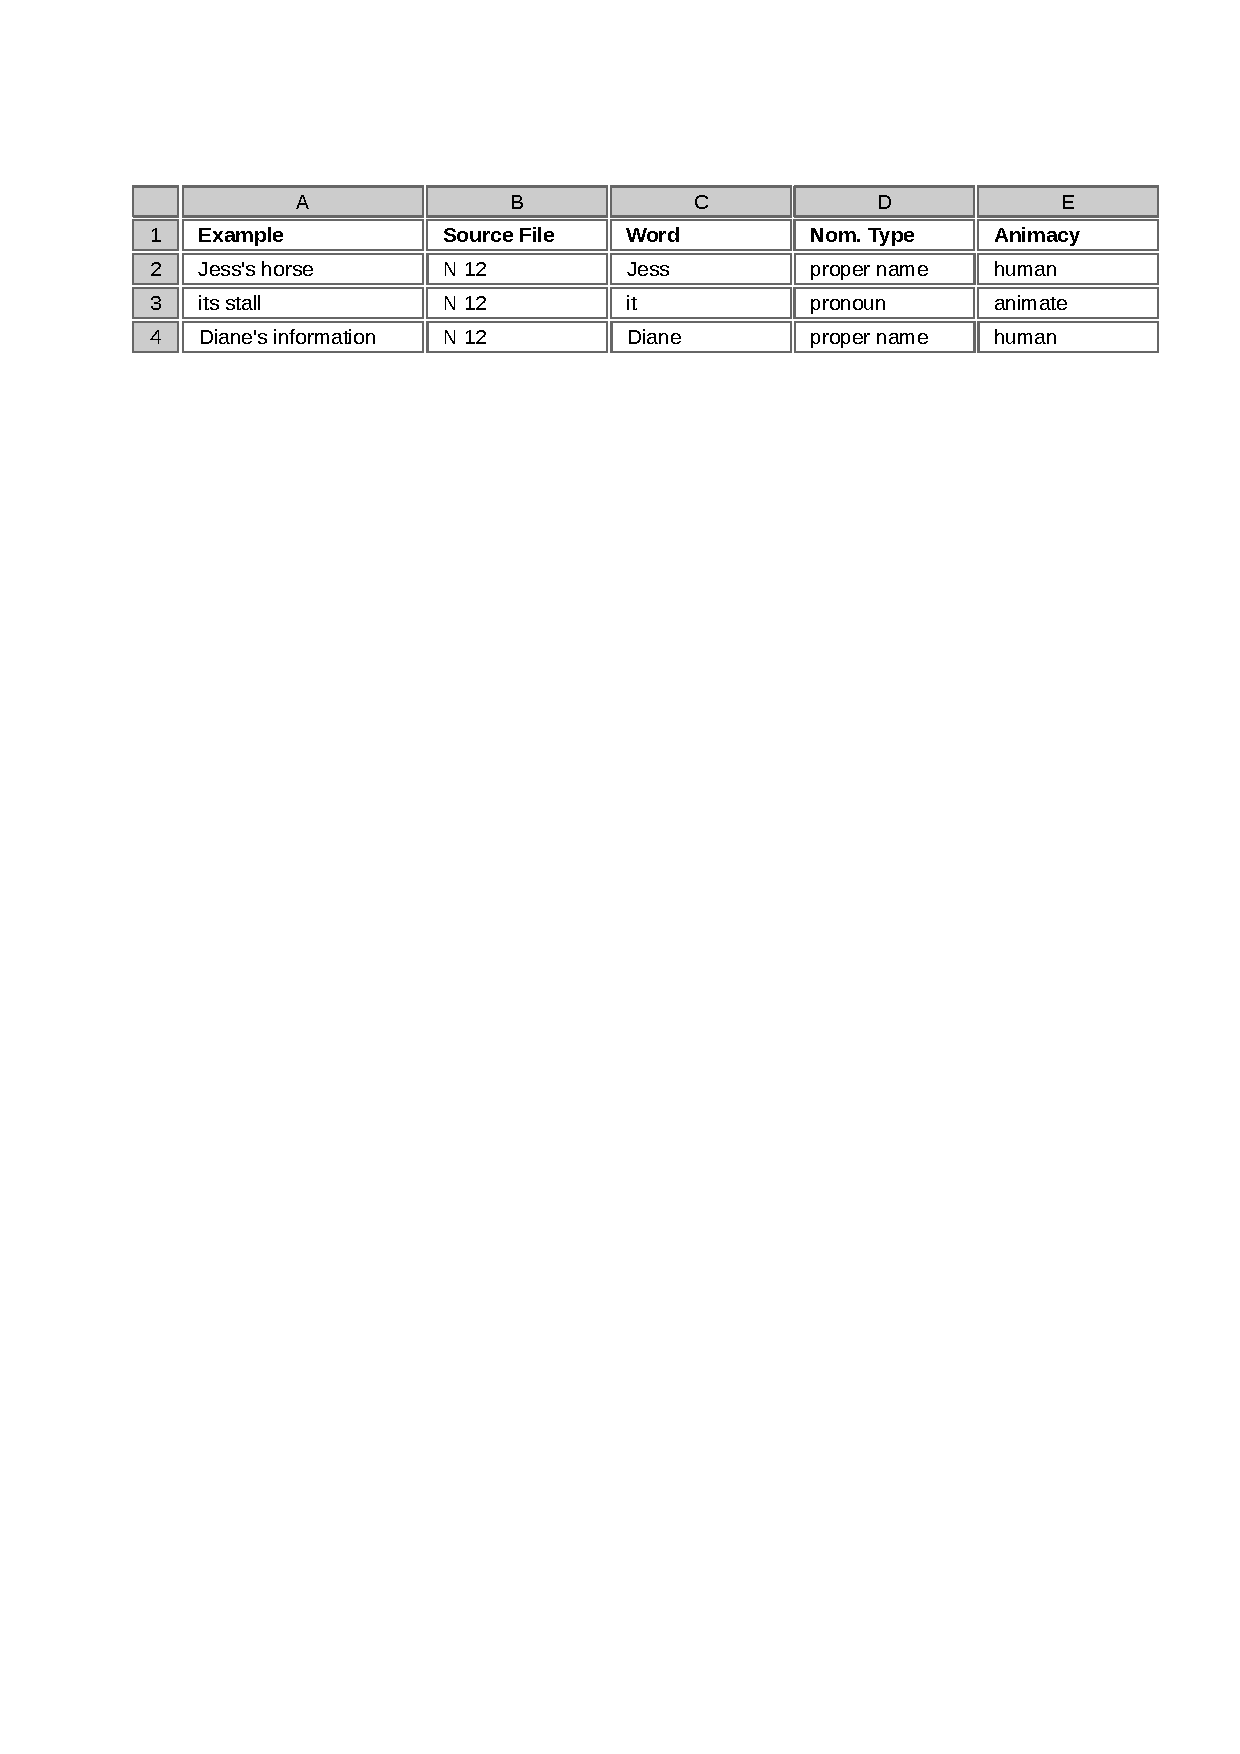
\includegraphics[width=\textwidth,keepaspectratio]{figures/storingdataright}
\end{figure}

The first line contains labels that tell us what information is found in each column respectively. This should include the example itself (either as shown in Figure \ref{fig:storingdataright}, or in the form of a KWIC concordance line) and meta-information such as what corpus and/or corpus file the example was extracted from. Crucially, it will include the relevant variables. Each subsequent line contains one observation (i.e., one hit and the appropriate values of each variable). This format -- one column for each variable, and one line for each example -- is referred to as a \textit{raw data table}. It is the standard way of recording measurements in all empirical sciences and we should adhere to it strictly, as it ensures that the \emph{structure} of the data is retained.

In particular, we should never store our data in summarized form, for example, as shown in Figure \ref{fig:storingdatawrong}.

\begin{figure}[!htbp]
\caption{Data stored in summarized form}
\label{fig:storingdatawrong}
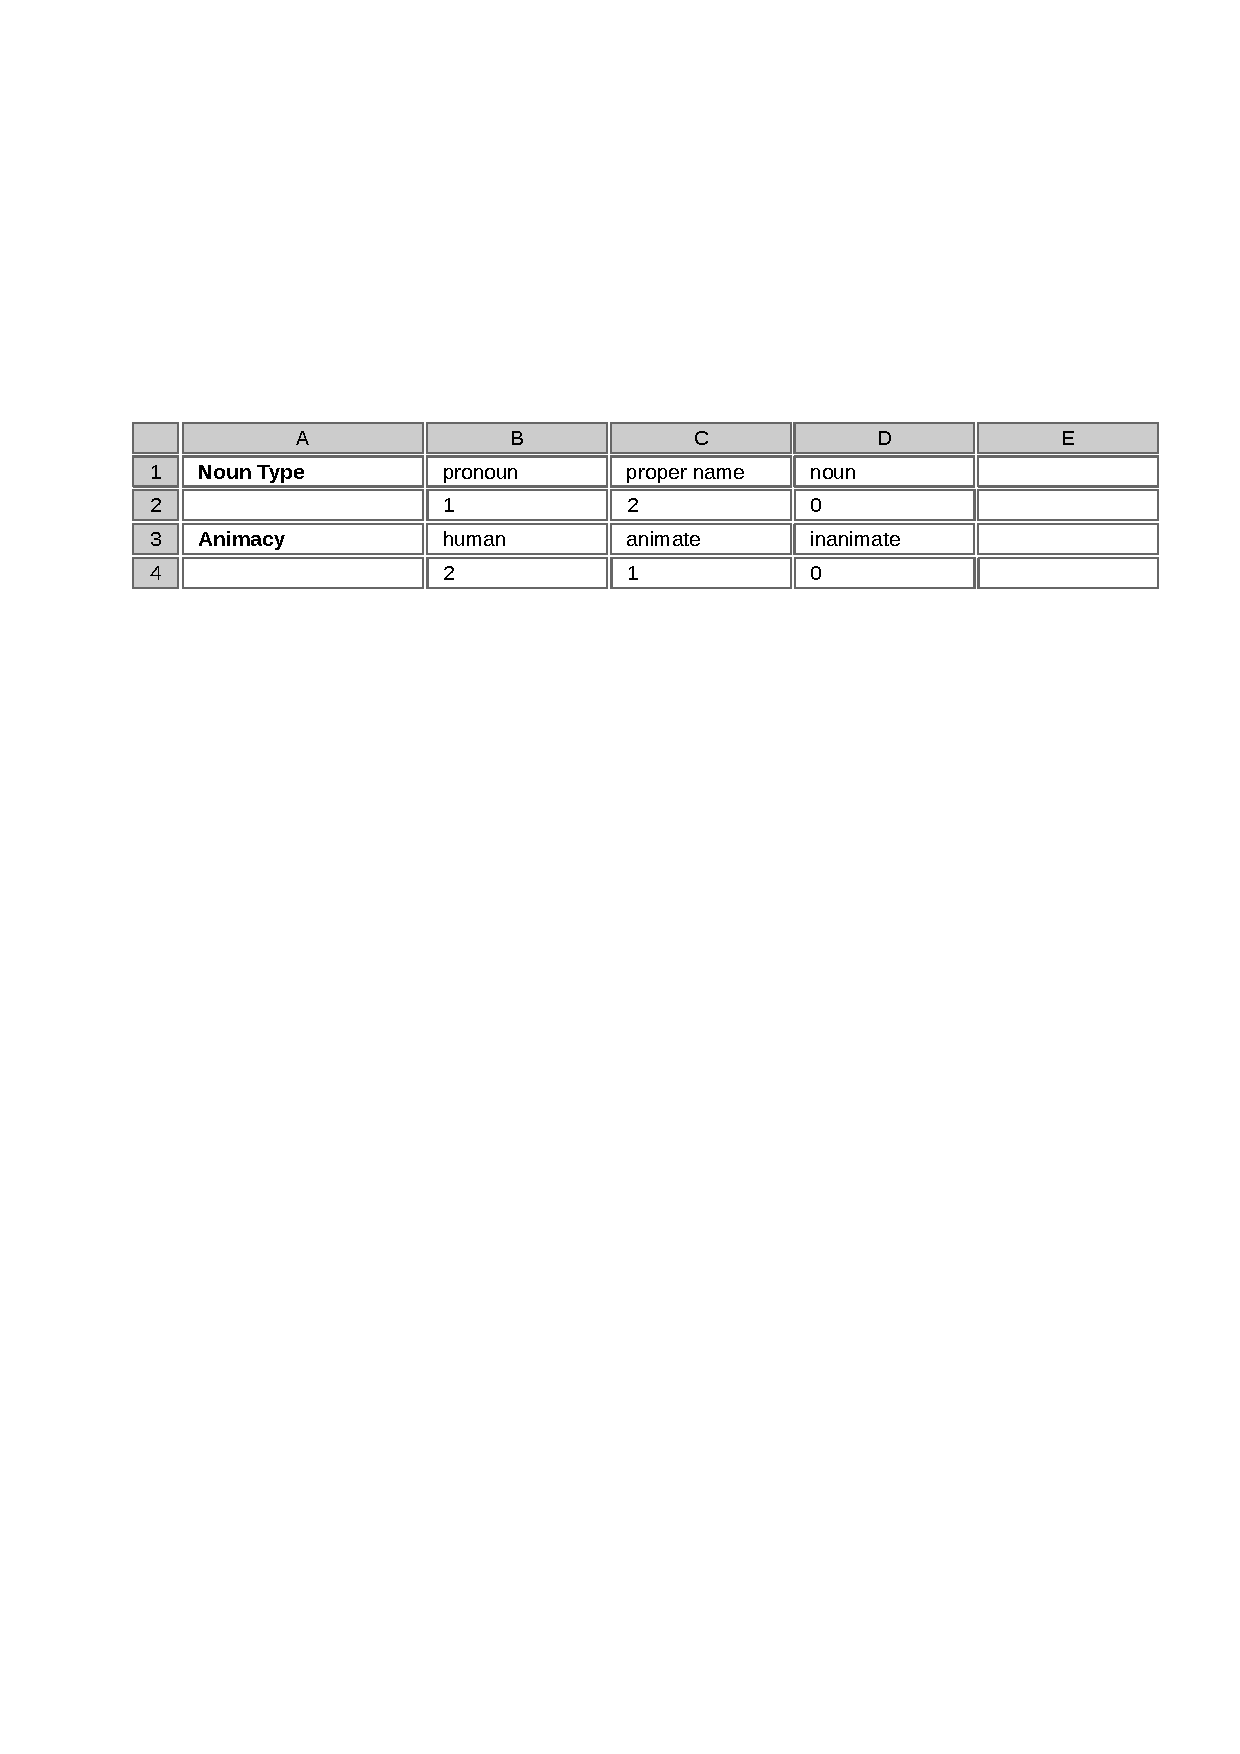
\includegraphics[width=\textwidth,keepaspectratio]{figures/storingdatawrong}
\end{figure}

There is simply no need to store data in this form -- if we need this type of summary, it can be created automatically from a raw data table like that in Figure \ref{fig:storingdataright} -- all major spreadsheet applications and statistical software packages have this functionality. What is more, statistics software packages require a raw data table of the type shown in Figure \ref{fig:storingdataright} as input for most statistical functions.

As mentioned above, however, the format of storage is not simply a practical matter, but a methodological one. If we did store our data in the form shown in Figure \ref{fig:storingdatawrong} straight away, we would destroy the relationship between the corpus hits and the different annotations applied to them and could never reconstruct them. In other words, we would have no way of telling which which combinations of variables actually occurred in the data. In Figure \ref{fig:storingdatawrong}, for example, we cannot tell whether the pronoun referred to one one of the human referents or to the animate referent. Even if we do not need to know these relationships for a given research project (or initially believe we do not), we should avoid this situation, as we do not know what additional questions may come up in the course of our research that do require this information.

Since quantitative analysis always requires a raw data table, we might conclude that it is the only useful way of recording our annotation decisions. However, there are cases where it may be more useful to record them in the form of annotations in (a copy of) the original corpus instead, i.e., analogously to automatically added annotations. For example, the information in Figure \ref{fig:storingdataright} could be recorded in the corpus itself in the same way that part-of-speech tags are, i.e., we could add an \textvv{Animacy} label to every nominal element in our corpus in the format used for POS tags by the original version of the BROWN corpus, as shown in (\ref{ex:storingdatainline}):

\begin{exe}
\ex \begin{minipage}[t]{\textwidth} \raggedright \texttt{the\_AT} \texttt{fact\_NN\_\textbf{abstract}} \texttt{that\_CS} \texttt{Jess's\_NP\$\_\textbf{human}} \texttt{horse\_NN\_\textbf{animate}} \texttt{had\_HVD} \texttt{not\_*} \texttt{been\_BEN} \texttt{returned\_VBN} \texttt{to\_IN} \texttt{its\_PP\$\_\textbf{animate}} \texttt{stall\_NN\_\textbf{inanimate}} \texttt{could\_MD} \texttt{indicate\_VB} \texttt{that\_CS} \texttt{Diane's\_NP\$\_\textbf{human}} \texttt{information\_NN\_\textbf{abstract}} \texttt{had\_HVD} \texttt{been\_BEN} \texttt{wrong\_JJ} \texttt{,\_,} \texttt{but\_CC} \texttt{Curt\_NP\_\textbf{human}} \texttt{didn't\_DOD*} \texttt{interpret\_VB} \texttt{it\_PPO\_\textbf{inanimate}} \texttt{this\_DT} \texttt{way\_NN\_\textbf{inanimate}} \texttt{.\_.} \end{minipage}
\label{ex:storingdatainline}
\end{exe}

From a corpus encoded in this way, we can alway create a raw data list like that in Figure \ref{fig:storingdataright} by searching for possessives and then separating the hits into the word itself, the \textvv{Part-of-Speech} label and the \textvv{Animacy} annotation (this can be done manually, or with the help of regular expressions in a text editor or with a few lines of code in a scripting language like Perl or Python).

The advantage would be that we, or other researchers, could also use our annotated data for research projects concerned with completely different research questions. Thus, if we are dealing with a variable that is likely to be of general interest, we should consider the possibility of annotating the corpus itself instead of first extracting the relevant data to a raw data table and annotating them afterwards.\footnote{The direct annotation of corpus files is rare in corpus linguistics, but it has become the preferred strategy in various fields concerned with qualitative analysis of textual data. There are open-source and commercial software packages dedicated to this task. They typically allow the user to define a set of annotation categories with appropriate codes, import a text file, and then assign the codes to a word or larger textual unit by selecting it with the mouse and then clicking a button for the appropriate code that is then added (often in XML format) to the imported text. This strategy has the additional advantage that one can view one's annotated examples in their original context (which may be necessary when annotating additional variables later). However, the available software packages are geared towards the analysis of individual texts and do not let the user to work comfortably with large corpora.}
